\documentclass[12pt,a4paper]{article}
\usepackage[UTF8]{ctex}
\usepackage{amsmath,amssymb}
\usepackage{listings}
\usepackage{xcolor}
\usepackage{hyperref}
\usepackage{geometry}
\usepackage{graphicx}
\geometry{margin=2.5cm}

\lstdefinestyle{python}{
  language=Python,
  basicstyle=\ttfamily\small,
  keywordstyle=\color{blue}\bfseries,
  commentstyle=\color{gray},
  stringstyle=\color{red},
  showstringspaces=false,
  breaklines=true,
  frame=single,
  backgroundcolor=\color{gray!10}
}

\title{GHZ State / GHZ 态}
\author{QuoNic}
\date{}

\begin{document}
\maketitle

\begin{center}
\textbf{Foundational / 基础} | 难度：中级 | 预计时间：10 分钟
\end{center}

\tableofcontents
\newpage

%% ============================================================
\section{为什么需要？}

GHZ 态是 Bell 态的多量子比特推广，是量子纠缠的另一种重要形式。

\subsection{经典局限}
\b\begin{itemize}
  \item 经典物理无法创建三个或更多粒子的完美关联
  \item 经典通信无法实现多方量子协议
\end{itemize}

\subsection{量子优势}
\b\begin{itemize}
  \item GHZ 态是量子纠错的基础资源
  \item 用于多方量子通信和量子秘密共享
  \item 是量子计算中常用的纠缠态
\end{itemize}

\subsection{实际应用}
\b\begin{itemize}
  \item 量子纠错（表面码、颜色码）
  \item 量子秘密共享（多方协议）
  \item 量子计算测试（多量子比特纠缠验证）
\end{itemize}

%% ============================================================
\section{快速上手}

\begin{lstlisting}[style=python]
from quonic import qgate, qshow
from quonic.gates import CX, H

# 创建 GHZ 态：(|000>+|111>)/sqrt(2)
qgate(H, 0)
qgate(CX, 0, 1)
qgate(CX, 1, 2)
qshow()
\end{lstlisting}

\textbf{预期输出}：
\begin{verbatim}
backend: native | shots: 1024
Result:
  |000>    512  ( 50.0%)  ####################
  |111>    512  ( 50.0%)  ####################
\end{verbatim}

%% ============================================================
\section{原理详解}

\subsection{电路图}

\begin{center}
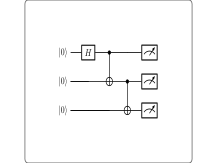
\includegraphics[width=0.7\textwidth]{../../images/ghz_circuit.svg}
\end{center}

\subsection{数学推导}

\textbf{Step 1: 初始状态}

三个量子比特都从 $|0\rangle$ 开始：
\begin{equation}
|\psi_0\rangle = |000\rangle
\end{equation}

\textbf{Step 2: Hadamard 门}

对 $q_0$ 施加 $H$ 门：
\begin{equation}
|\psi_1\rangle = \frac{|0\rangle + |1\rangle}{\sqrt{2}} \otimes |00\rangle = \frac{|000\rangle + |100\rangle}{\sqrt{2}}
\end{equation}

\textbf{Step 3: CNOT 门链}

CNOT$(q_0, q_1)$ 和 CNOT$(q_1, q_2)$ 创建三量子比特纠缠：
\begin{equation}
|\psi_2\rangle = \frac{|000\rangle + |111\rangle}{\sqrt{2}}
\end{equation}

\textbf{Step 4: 测量概率}

\b\begin{itemize}
  \item $P(|000\rangle) = 0.5$
  \item $P(|111\rangle) = 0.5$
  \item 其他态的概率为 0
\end{itemize}

\subsection{几何解释}

GHZ 态是三量子比特的最大纠缠态。在 Bloch 球上，三个量子比特的状态完全关联——测量一个就能确定其他两个。

%% ============================================================
\section{代码详解}

\begin{lstlisting}[style=python]
from quonic import qgate, qshow
from quonic.gates import CX, H

qgate(H, 0)       # H gate on q0: create superposition
qgate(CX, 0, 1)   # CNOT: entangle q0 and q1
qgate(CX, 1, 2)   # CNOT: entangle q1 and q2
qshow()            # measure and display
\end{lstlisting}

\subsection{API 说明}

\begin{center}
\begin{tabular}{|l|l|l|}
\hline
\textbf{API} & \textbf{参数} & \textbf{说明} \\
\hline
\texttt{qgate(H, 0)} & H: Hadamard 门 & 创建叠加态 \\
\hline
\texttt{qgate(CX, 0, 1)} & CX: CNOT 门 & 创建两量子比特纠缠 \\
\hline
\texttt{qgate(CX, 1, 2)} & CX: CNOT 门 & 扩展到三量子比特 \\
\hline
\end{tabular}
\end{center}

%% ============================================================
\section{进阶用法}

\subsection{场景 1：N 量子比特 GHZ 态}

\begin{lstlisting}[style=python]
# N-qubit GHZ state
n = 5
qgate(H, 0)
for i in range(n - 1):
    qgate(CX, i, i + 1)
qshow()
\end{lstlisting}

\subsection{场景 2：GHZ 态的保真度测试}

\begin{lstlisting}[style=python]
# Fidelity test with noise
qgate(H, 0)
qgate(CX, 0, 1)
qgate(CX, 1, 2)
qshow(noise=0.05)
\end{lstlisting}

\subsection{场景 3：GHZ 态用于量子纠错}

\begin{lstlisting}[style=python]
# GHZ state for error correction
# Encode logical qubit in GHZ state
qgate(H, 0)
qgate(CX, 0, 1)
qgate(CX, 1, 2)
# Syndrome measurement
qgate(CX, 0, 3)
qgate(CX, 1, 3)
qshow()
\end{lstlisting}

%% ============================================================
\section{适用场景}

\subsection{量子纠错}

GHZ 态是量子纠错码的基础资源。表面码和颜色码都使用多量子比特纠缠来保护量子信息。

\subsection{量子秘密共享}

在量子秘密共享协议中，GHZ 态用于将秘密分发给多个参与方。只有所有参与方合作才能恢复秘密。

\subsection{量子计算测试}

GHZ 态是测试量子硬件多量子比特纠缠能力的标准基准。

%% ============================================================
\section{常见问题}

\subsection{GHZ 态和 Bell 态有什么区别？}

Bell 态是 2 量子比特纠缠，GHZ 态是 3+ 量子比特纠缠。GHZ 态是 Bell 态的推广。

\subsection{为什么 GHZ 态只有 |000> 和 |111>？}

因为 CNOT 门链将 $q_0$ 的状态传播到所有量子比特。如果 $q_0$ 是 $|0\rangle$，所有量子比特都是 $|0\rangle$；如果 $q_0$ 是 $|1\rangle$，所有量子比特都是 $|1\rangle$。

\subsection{GHZ 态的纠缠特性是什么？}

GHZ 态是最大纠缠态——测量一个量子比特会瞬间确定所有其他量子比特的状态。

%% ============================================================
\section{学习路径}

\subsection{前置知识}
\b\begin{itemize}
  \item Bell 态（2 量子比特纠缠）
  \item CNOT 门和 Hadamard 门
  \item 量子测量
\end{itemize}

\subsection{继续学习}
\b\begin{itemize}
  \item 量子纠错码（表面码、颜色码）
  \item 量子秘密共享
  \item 多量子比特纠缠验证
\end{itemize}

%% ============================================================
\section{完整示例代码}

\subsection{示例 1：基本 GHZ 态}

\begin{lstlisting}[style=python]
from quonic import qgate, qshow
from quonic.gates import CX, H

qgate(H, 0)
qgate(CX, 0, 1)
qgate(CX, 1, 2)
qshow()
\end{lstlisting}

\subsection{示例 2：带噪声的 GHZ 态}

\begin{lstlisting}[style=python]
from quonic import qgate, qshow
from quonic.gates import CX, H

qgate(H, 0)
qgate(CX, 0, 1)
qgate(CX, 1, 2)
qshow(noise=0.05)
\end{lstlisting}


\section{下载}

\begin{itemize}
  \item [ghz.py](https://github.com/ChrisLee0721/QuoNic/blob/main/examples/ghz/ghz.py)
\end{itemize}

\end{document}
